\documentclass[red]{beamer}

\mode<presentation>
\usetheme{Berkeley}

% define your own colours:
\definecolor{Red}{rgb}{1,0,0}
\definecolor{Blue}{rgb}{0,0,1}
\definecolor{Green}{rgb}{0,1,0}
\definecolor{magenta}{rgb}{1,0,.6}
\definecolor{lightblue}{rgb}{0,.5,1}
\definecolor{lightpurple}{rgb}{.6,.4,1}
\definecolor{gold}{rgb}{.6,.5,0}
\definecolor{orange}{rgb}{1,0.4,0}
\definecolor{hotpink}{rgb}{1,0,0.5}
\definecolor{newcolor2}{rgb}{.5,.3,.5}
\definecolor{newcolor}{rgb}{0,.3,1}
\definecolor{newcolor3}{rgb}{1,0,.35}
\definecolor{darkgreen1}{rgb}{0, .35, 0}
\definecolor{darkgreen}{rgb}{0, .6, 0}
\definecolor{darkred}{rgb}{.75,0,0}
\xdefinecolor{olive}{cmyk}{0.64,0,0.95,0.4}
\xdefinecolor{purpleish}{cmyk}{0.75,0.75,0,0}
\useoutertheme[subsection=false]{smoothbars}
\setbeamercolor{block title}{bg=black,fg=white}

%% \renewcommand{\qedsymbol}{$\blacksquare$}

\newenvironment<>{varblock}[2][.9\textwidth]{%
  \setlength{\textwidth}{#1}
  \begin{actionenv}#3%
    \def\insertblocktitle{#2}%
    \par%
    \usebeamertemplate{block begin}}
  {\par%
    \usebeamertemplate{block end}%
  \end{actionenv}}

% \usefonttheme[onlymath]{serif}
% \usepackage{fontspec} 
% \defaultfontfeatures{Mapping=tex-text} 
% \setsansfont[Ligatures={Common}]{Futura}
% \setmonofont[Scale=0.8]{Monaco} 
\usepackage{enumitem}
% \newlist{wideenum}{enumerate}{4}
% \setlist[wideenum]{label*=\arabic*.,wide}

\usepackage{mathptmx}
\usepackage[scaled=0.9]{helvet}
\usepackage{courier}

\usepackage{soul}
\usepackage{subfigure}
\usepackage{multicol}
\usepackage{amssymb,amsmath}
\usepackage{epsfig}
\usepackage{graphicx}
\usepackage[all,knot]{xy}
\xyoption{arc}
\usepackage{url}
\usepackage{multimedia}
\usepackage{hyperref}
\usepackage{setspace}
\usepackage{breqn}
\usepackage{anyfontsize}
\usepackage{textpos}
\usepackage{bibentry}
\usepackage{stmaryrd}
\usepackage{tikz}
\usepackage{tcolorbox}
\usepackage{bm}
\usepackage[geometry]{ifsym}
%% \usepackage[showframe=true]{geometry}
% \usepackage{enumitem}
% \usepackage{lipsum}
% \setlist[itemize]{leftmargin=*}

% \newcommand\crule[3][black]{\textcolor{#1}{\rule{#2}{#3}}}

%% \newcommand{\newsymbol}{
%% \begin{tikzpicture}
%% \filldraw[fill=black,draw=red] circle (3pt);
%% \end{tikzpicture}
%% }

% \usepackage{xcolor}
% \newif\ifgooditem
% \gooditemtrue
% \newcommand\gooditem{\gooditemtrue\item}
% \newcommand\baditem{\gooditemfalse\item}

\newtcolorbox{mybox}[3][]
{
  colframe = black,
  colback  = #2!10,
  coltitle = #2!20!white,  
  title    = #3,
  #1,
}
\setitemize{label=\usebeamerfont*{itemize item}%
  \usebeamercolor[fg]{itemize item}
  \usebeamertemplate{itemize item}}

% \setbeamertemplate{itemize items}[square]
%%%%%%%%%%%%%%%%%%%%%%%%%%%%%%%%%%%%%%%%%%%%%%%%%%%%%%%%%%%%
%
% Custom Includes
%
%%%%%%%%%%%%%%%%%%%%%%%%%%%%%%%%%%%%%%%%%%%%%%%%%%%%%%%%%%%%
% \newcommand{\SurfELIntX}{\tvInt{\partial \Omega^{e}_l}{}{s}}
\newcommand{\Mmat}[2]{\mathbb{M}^e[#1,#2]}
\newcommand{\Dmat}[2]{\mathbb{D}^e_k[#1,#2]}
\newcommand{\Dmatx}[2]{\mathbb{D}^e_x[#1,#2]}
\newcommand{\Dmaty}[2]{\mathbb{D}^e_y[#1,#2]}
\newcommand{\Smat}[2]{\mathbb{S}^e_k[#1,#2]}
\newcommand{\Smatx}[2]{\mathbb{S}^e_x[#1,#2]}
\newcommand{\Smaty}[2]{\mathbb{S}^e_y[#1,#2]}
\newcommand{\Fmat}[2]{\mathbb{F}^e_l[#1,#2]}
\newcommand{\Ftmat}[2]{\widetilde{\mathbb{F}}^e_{kl}[#1,#2]}
\newcommand{\Ftmatx}[2]{\widetilde{\mathbb{F}}^e_{xl}[#1,#2]}
\newcommand{\Ftmaty}[2]{\widetilde{\mathbb{F}}^e_{yl}[#1,#2]}
\newcommand{\utrace}{ \widetilde{u} }
\newcommand{\qtrace}{ \widetilde{\tv q} }
\newcommand{\uhat}{\Hat u}
\newcommand{\fhat}{\Hat f}
\newcommand{\qhat}{\Hat {\tv q}}
\newcommand{\umodes}[1]{\uhat^e[{#1}]}
\newcommand{\qmodesx}[1]{\qhat^e_x[{#1}]}
\newcommand{\qmodesy}[1]{\qhat^e_y[{#1}]}
\newcommand{\fmodes}[1]{\fhat^e[{#1}]}
\newcommand{\qmodes}[1]{\qhat^e_k[{#1}]}
\newcommand{\utmodes}[1]{\widehat{\widetilde{u}}{}^l[{#1}]}
\newcommand{\qtmodes}[1]{\widehat{\widetilde{\tv q}}{}^l_k[{#1}]}
\newcommand{\qtmodesx}[1]{\widehat{\qtrace}^l_x[{#1}]}
\newcommand{\qtmodesy}[1]{\widehat{\qtrace}^l_y[{#1}]}
\newcommand{\tvhat}[1]{\tv{\Hat{#1}}} 
\newcommand{\tv}[1]{\boldsymbol{#1}}
\newcommand{\tvf}[1]{\uline{\textbf{#1}}}
\newcommand{\tvInt}[3]{\int_{#1}^{#2} \mathrm{d}#3 \,}
\newcommand{\VolIntX}{\tvInt{\Omega}{}{\tv x}}
\newcommand{\SurfIntX}{\tvInt{\partial \Omega}{}{s}}
\newcommand{\VolEIntX}{\tvInt{\Omega^{e}}{}{\tv x}}
\newcommand{\SurfEIntX}{\tvInt{\partial \Omega^{e}}{}{s}}
\newcommand{\tvPartial}[2]{ \frac{\partial#1}{\partial#2} }
\newcommand{\tvDeriv}[2]{ \frac{d#1}{d#2} }
\newcommand{\tvSDeriv}[2]{ \frac{d^2#1}{{d#2}^2} }
\newcommand{\mani}{\mathcal{M}}
\newcommand{\tess}{\mathcal{T}\left(\Omega \right)}
\newcommand{\fol}{\left \{ \Sigma_t \right \} }
\newcommand{\hyp}{ \Sigma_{t} }
\newcommand{\eqnref}[1]{ Equation (\ref{#1}) }
\newcommand{\barD}{ \bar{D} }
\newcommand{\barGam}{ \bar{\gamma} }
\newcommand{\barS}{ \bar{s} }
\newcommand{\barA}{ \bar{A} }
\newcommand{\barM}{ \bar{m} }
\newcommand{\barGAM}{ \bar{\Gamma} }
\newcommand{\barR}{ \bar{R} }
\newcommand{\barP}{ \bar{p} }
\newcommand{\barE}{ \bar{E} }
\newcommand{\barL}{ \bar{L} }
\newcommand{\barN}{ \bar{N} }
\newcommand{\barDelta}{ \bar{\Delta}}
\newcommand{\barATT}{ \bar{A}_{TT}}


% DOUBLE BRACES IN DISCONTINUOUS GALERKIN METHODS
% See http://tex.stackexchange.com/questions/252648/left-right-double-curly-brace-blackboard-bold-symbol
% Usage:
% \def\test#1{#1|xxx}
% $\dgal*{\test{}}$
% $\dgal*{\test{\big}}$
% $\dgal*{\test{\Big}}$
% $\dgal*{\test{\bigg}}$
% $\dgal*{\test{\Bigg}}$
% $\dgal{xxx}$
% $\dgal[\big]{xxx}$
% $\dgal[\Big]{xxx}$
% $\dgal[\bigg]{xxx}$
% $\dgal[\Bigg]{xxx}$

\usepackage{xparse}

\NewDocumentCommand{\dgal}{sO{}m}{%
  \IfBooleanTF{#1}
    {\dgalext{#3}}
    {\dgalx[#2]{#3}}%
}

\NewDocumentCommand{\dgalext}{m}{%
  \sbox0{%
    \mathsurround=0pt % just for safety
    $\left\{\vphantom{#1}\right.\kern-\nulldelimiterspace$%
  }%
  \sbox2{\{}%
  \ifdim\ht0=\ht2
    \{\kern-.45\wd2 \{#1\}\kern-.45\wd2 \}%
  \else
    \left\{\kern-.5\wd0\left\{#1\right\}\kern-.5\wd0\right\}%
  \fi
}

\NewDocumentCommand{\dgalx}{om}{%
  \sbox0{\mathsurround=0pt$#1\{$}%
  \sbox2{\{}%
  \ifdim\ht0=\ht2
    \{\kern-.45\wd2 \{#2\}\kern-.45\wd2 \}%
  \else
    \mathopen{#1\{\kern-.5\wd0 #1\{}
    #2
    \mathclose{#1\}\kern-.5\wd0 #1\}}
  \fi
}


\usepackage{booktabs}
\newcommand{\ra}[1]{\renewcommand{\arraystretch}{#1}}


%%%%%%%%%%%%%%%%%%%%%%%%%%%%%%%%%%%%%%%%%%%%%%%%%%%%%%%%%%%%
%
% Title Page
%
%%%%%%%%%%%%%%%%%%%%%%%%%%%%%%%%%%%%%%%%%%%%%%%%%%%%%%%%%%%%

\newcommand*\leftright[2]{%
  \leavevmode
  \rlap{#1}%
  \hspace{0.25\linewidth}%
  #2}

\title[\phantom{Binary Neutron} BNS Simulations]{\textbf{Binary Neutron Star Simulations: \\ New Tools and Insights} }
\author{Trevor Vincent}
% \institute{{\\ \small Committee}\\ \vspace{.05cm} \leftright{Dr.Harald Pfeiffer}{Dr. Charles Dyer} \\
% \leftright{\hspace{.275cm} Dr. Ue-Li Pen}{Dr. Robin Marjoribanks} }
\institute{{\\ \scriptsize Committee}\\ \vspace{.05cm}\begin{minipage}[t]{0.4\textwidth}\begin{center}\begin{itemize}[noitemsep]
% \begin{multicols}{2}
    \item[] \phantom{te}Prof. John Sipe
    \item[] \phantom{te}Prof. Harald Pfeiffer
    \item[] \phantom{te}Prof. Charles Dyer
% \item[] 
    \item[] \phantom{te}Prof. Amar Vutha
    %% \item[] Dr. Robin Marjoribanks
% \end{multicols}
\end{itemize} \end{center}\end{minipage}}
\date{ \\\scriptsize PhD Internal Defense \vspace{.10cm}\\ Physics Department \vspace{.10cm}\\ University of Toronto\\ \vspace{.10cm}\today}

\begin{document}


\frame{\titlepage}
\section{Background}
\subsection{GW170817}
\frame{
\frametitle{GW170817: Welcome to the Multi-messenger Era}
\begin{columns}
  \begin{column}{.48\textwidth}
    \begin{mybox}{white}{\centering \scriptsize Event}
      \scriptsize
      %% \begin{itemize}[label=\FilledSmallSquare]
          {\bf Object}: BNS \\
     {\bf Total mass}: $2.74M_\odot$ \\
     {\bf Distance}: 40 Mpc \\
     {\bf GW Radiation}: $0.025M_\odot$ \\
     {\bf GW Duration}: 100 s \\
     {\bf Galaxy}: NGC-4993
    %% \end{itemize}
\end{mybox}
\begin{mybox}{white}{\centering \scriptsize Science}
  \scriptsize
    \begin{itemize}[label=\FilledSmallSquare]
    \item short gamma ray burst
    \item kilonova (optical $\rightarrow$ radio)
    \item neutrinos (none-found)
    \item r-process nuclei 
    \item speed of gravity
    \item EOS constraints
    \item $H_0$ constraints
    \end{itemize}
\end{mybox}    
%% \vspace{1cm}
%% Candidate Systems
%% \begin{itemize}
%% \scriptsize 
%% \item[\blacksquare]\scriptsize Binary Neutron Star (NS-NS)
%% \item[\blacksquare]\scriptsize Binary Black Holes (BH-BH)
%% \item[\blacksquare]\scriptsize Neutron Star - Black Hole (NS-BH)
%% \end{itemize}
  \end{column}
  \begin{column}{.48\textwidth}
    %% \end{mybox}
\begin{mybox}{white}{\centering \scriptsize arXiv:1710.05833}
    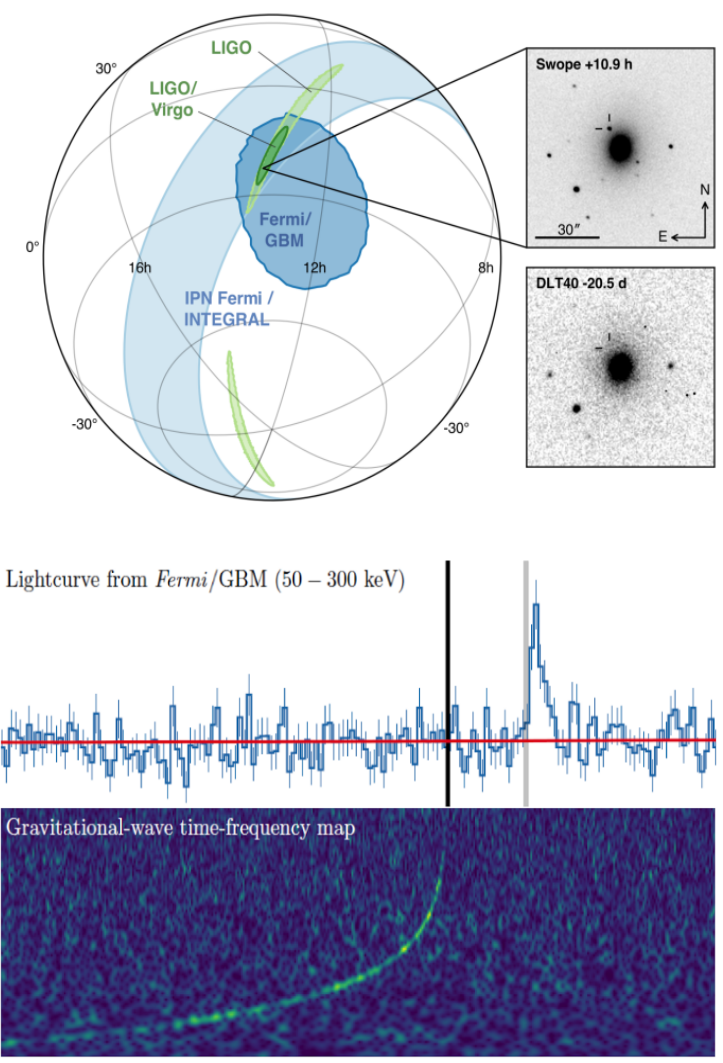
\includegraphics[width=1.05\textwidth]{pictures/attempt1.png} \\
   %% \text{\tiny \phantom{asdfasdfasdfasdf} [arXiv:1710.05833]}
   %% 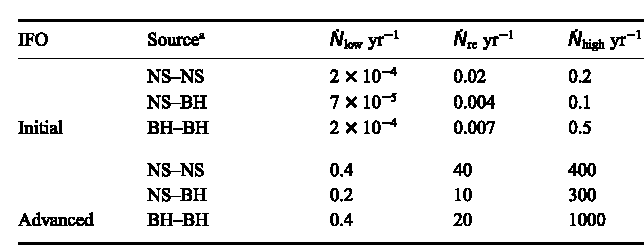
\includegraphics[width=\textwidth]{pictures/abadie.pdf} \\
    %% \centering{\text{ \tiny [Abadie et al; 1003.2480]}}
\end{mybox}    
\end{column}
\end{columns}
%% \begin{mybox}{white}{\centering \scriptsize Expected NSNS Detection Rate}
  %% More than 10+ NSNS mergers detected per \bf{week}
%% \end{mybox}
}

%% \frame{\titlepage}
%% \section{Background}
\subsection{Next Generation GW Astronomy}
\frame{
\frametitle{Next-Generation Gravitational Wave Astronomy}
\begin{columns}
  \begin{column}{.48\textwidth}
    Detector network by $\approx 2026$
    \begin{itemize}[label=\FilledSmallSquare]
      %% \scriptsize
      %% \item dingdong
    \item LIGO A+ (Washington State)
    \item LIGO A+ (Louisiana)
    \item aVIRGO (Italy)
    \item GEO-HF (Germany)
    \item KAGRA (Japan)
    \item LIGO-India
    \end{itemize}
%% \vspace{1cm}
%% Candidate Systems
%% \begin{itemize}
%% \scriptsize 
%% \item[\blacksquare]\scriptsize Binary Neutron Star (NS-NS)
%% \item[\blacksquare]\scriptsize Binary Black Holes (BH-BH)
%% \item[\blacksquare]\scriptsize Neutron Star - Black Hole (NS-BH)
%% \end{itemize}
  \end{column}
  \begin{column}{.48\textwidth}
\centering{\text{\tiny [Sathyaprakash 2014]}}
   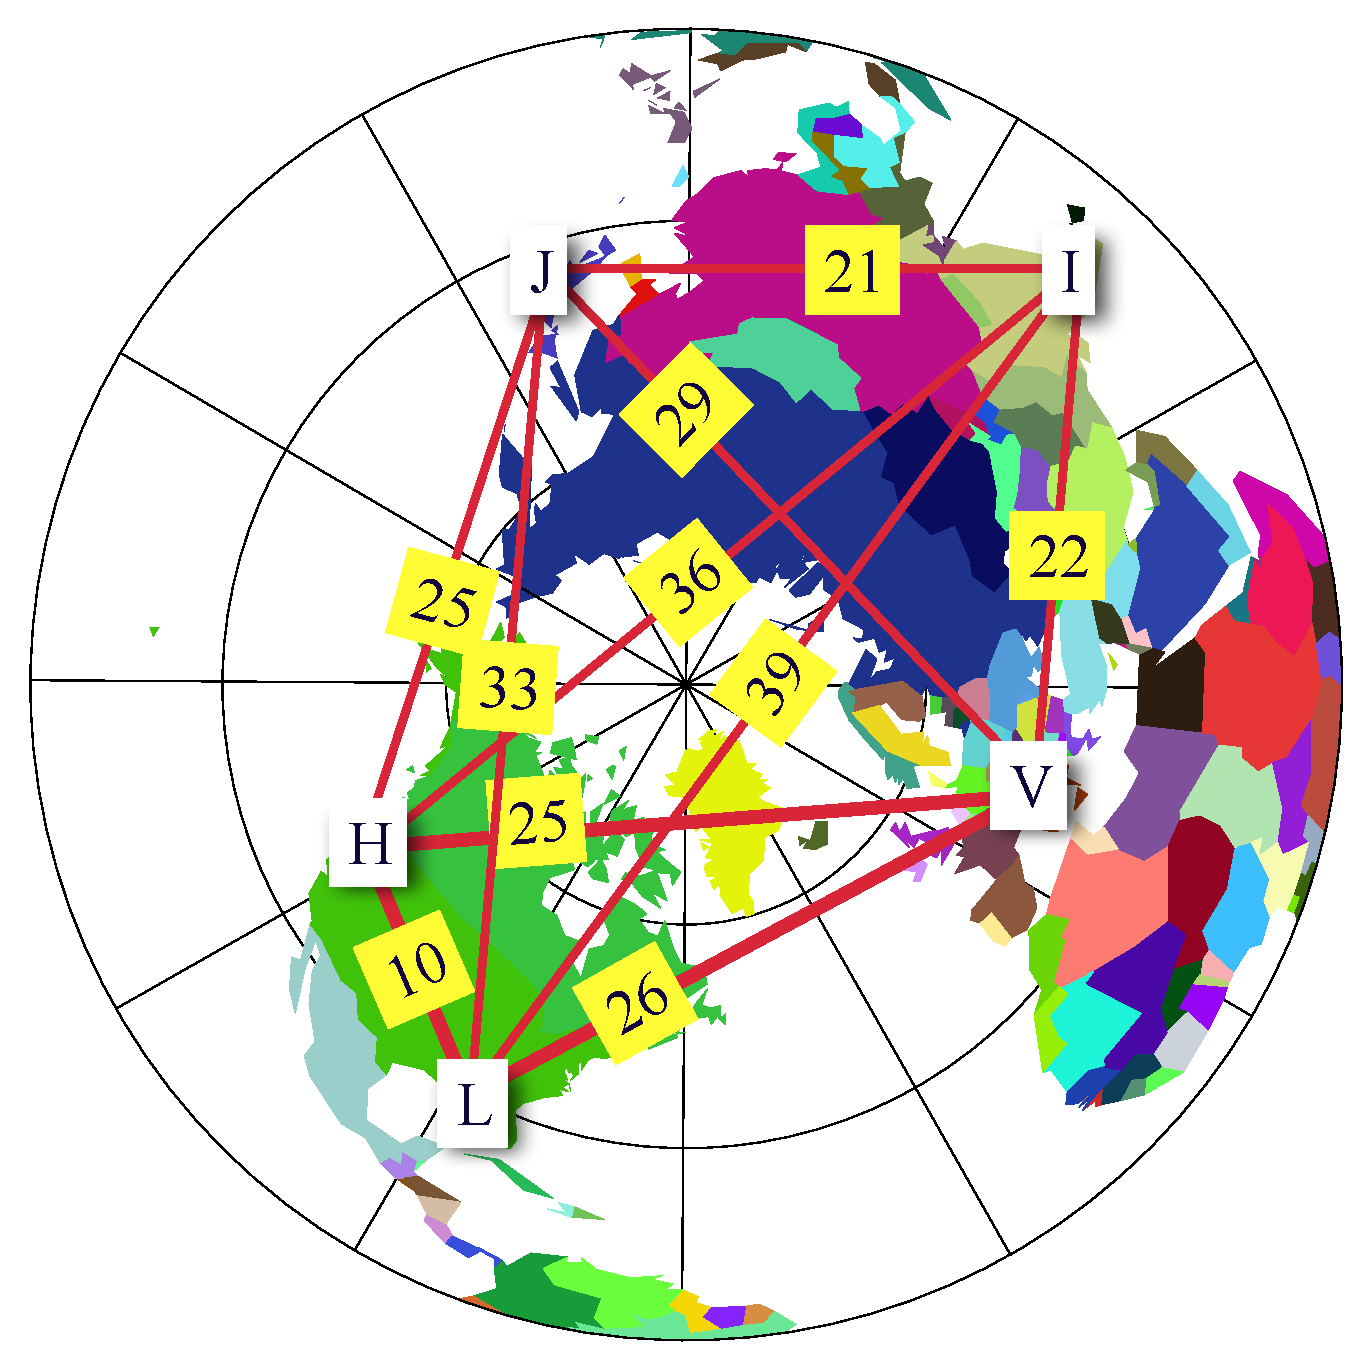
\includegraphics[width=.9\textwidth]{pictures/worldwide.pdf} \\
   %% 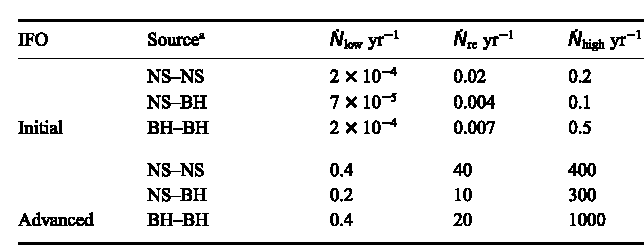
\includegraphics[width=\textwidth]{pictures/abadie.pdf} \\
    %% \centering{\text{ \tiny [Abadie et al; 1003.2480]}}
  \end{column}
\end{columns}

\begin{mybox}{white}{\centering \scriptsize Expected NSNS Detection Rate}
  More than 10+ NSNS mergers detected per \bf{week}
\end{mybox}
}


\subsection{Numerical Relativity}
\frame{
\frametitle{Numerical Relativity}
\begin{columns}
  \begin{column}{.48\textwidth}
    Detector network by $\approx 2026$
    \begin{itemize}[label=\FilledSmallSquare]
      %% \scriptsize
      %% \item dingdong
    \item LIGO A+ (Washington State)
    \item LIGO A+ (Louisiana)
    \item aVIRGO (Italy)
    \item GEO-HF (Germany)
    \item KAGRA (Japan)
    \item LIGO-India
    \end{itemize}
%% \vspace{1cm}
%% Candidate Systems
%% \begin{itemize}
%% \scriptsize 
%% \item[\blacksquare]\scriptsize Binary Neutron Star (NS-NS)
%% \item[\blacksquare]\scriptsize Binary Black Holes (BH-BH)
%% \item[\blacksquare]\scriptsize Neutron Star - Black Hole (NS-BH)
%% \end{itemize}
  \end{column}
  \begin{column}{.48\textwidth}
\centering{\text{\tiny [Sathyaprakash 2014]}}
   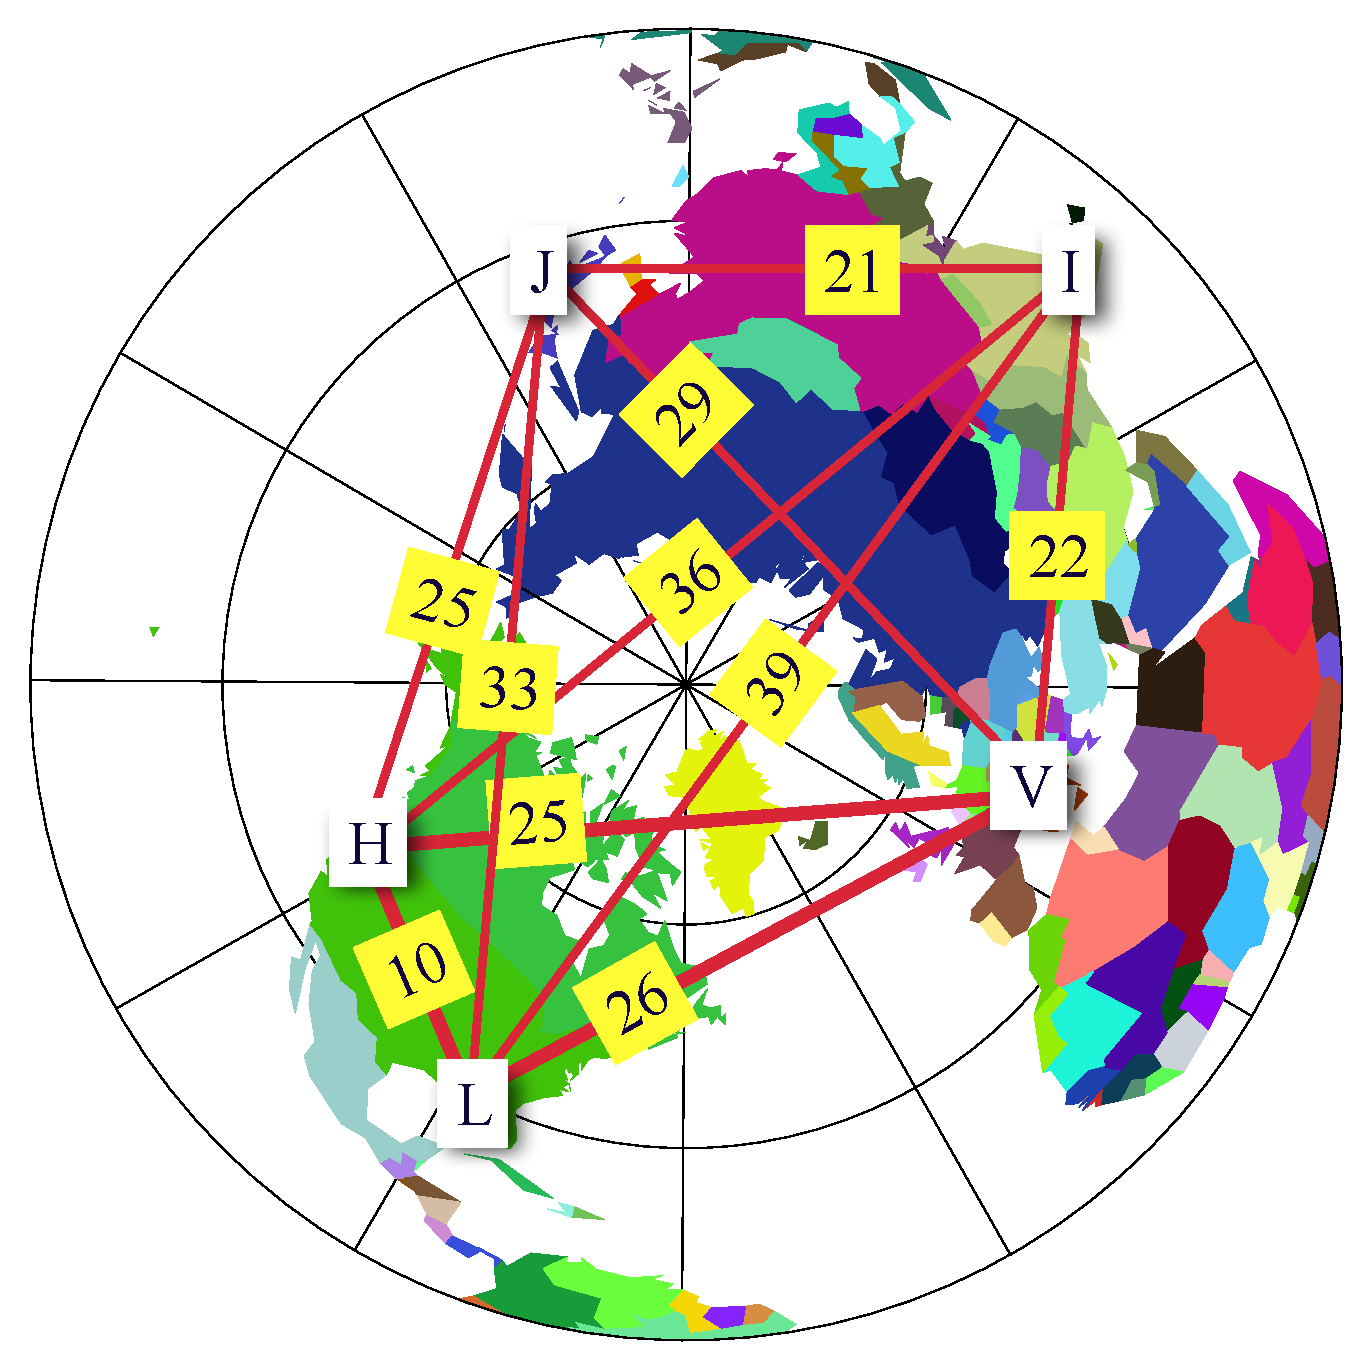
\includegraphics[width=.9\textwidth]{pictures/worldwide.pdf} \\
   %% 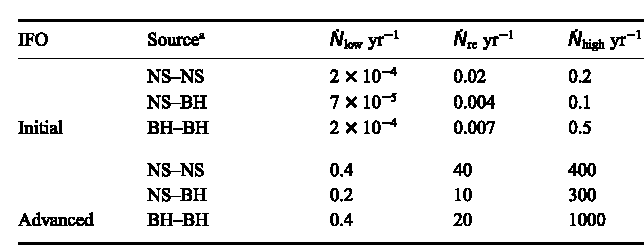
\includegraphics[width=\textwidth]{pictures/abadie.pdf} \\
    %% \centering{\text{ \tiny [Abadie et al; 1003.2480]}}
  \end{column}
\end{columns}

\begin{mybox}{white}{\centering \scriptsize Expected NSNS Detection Rate}
  More than 10+ NSNS mergers detected per \bf{week}
\end{mybox}
}

%% \frame{\titlepage}
\section{Chapter 1}
\subsection{New Code for NR}
\frame{
  \frametitle{Solving Non-linear Elliptic Equations}
}
%% \subsection{Code Overview}
\frame{
 \frametitle{Code Overview}
%% \begin{figure}
%%   \centering
%%   \begin{adjustbox}{width=.45\textwidth,trim=15 0 0 0, clip=true}
%% \begin{tikzpicture}[node distance=.25cm, auto]  
%% \tikzset{
%%     myCnode/.style={rectangle,rounded corners,draw=black, top color=white, bottom color=yellow!50,very thick, inner sep=1em, minimum size=3em, text centered},
%%     mySnode/.style={rectangle,rounded corners,draw=black, top color=white, bottom color=cyan!50,very thick, inner sep=1em, minimum size=3em, text centered},
%%     myarrow/.style={->, line width=1.3mm},
%%     myDarrow/.style={-, line width=1.3mm, dashed},
%%     myDarrow2/.style={->, line width=1.3mm, dashed},
%%     myBarrow/.style={-, line width=1.3mm},
%%     mylabel/.style={text width=8em, text centered} 
%%   }
%% \node[myCnode] (l1) {\Large   \,Level L\,};
%% \node[below=1cm of l1] (dummy) {}; 
%% \node[mySnode, right=of dummy] (l2) {\Large  Surrogate};
%% \node[below=1cm of l2] (dummy1) {}; 
%% \node[myCnode, right=of dummy1] (l3) {\Large  Level L-1};
%% \node[mylabel, left=.9cm of l2] (label1) {\Large   Coarsen};
%% \node[mylabel, left=.9cm of l3] (label1) {\Large   Enforce \break \\\vspace{-.4cm} 2:1 balance};
%% \node[below=3cm of l3] (dummy2) {}; 
%% \node[myCnode, right=.625cm of dummy2] (l4) {\Large  Level 0};
%% \node[myCnode, right=.86cm of l3] (l5) {\Large  Level L-1};
%% \node[above=2cm of l4] (dummydummy1) {};
%% \node[above=.5cm of l4] (dummydummy2) {};
%% \node[above=1cm of l5] (dummy4) {}; 
%% \node[mySnode, right=4.15cm of l2] (l6) {\Large  Surrogate};
%% \node[above=1cm of l6] (dummy5) {}; 
%% \node[myCnode, right=of dummy5] (l7) {\Large  \,Level L\,};
%% \node[right=of l7] (dummy51) {};
%% \node[mylabel, right=.7cm of l5] (label1) {\Large  Undo \break \\\vspace{-.4cm} 2:1 balance};
%% \node[mylabel, right=.7cm of l6] (label1) {\Large  Refine};
%% % for going down arrow
%% \node[left=of l1] (dummy61) {}; 
%% \node[below=1cm of l3] (dummyf) {}; 
%% \node[left=of l3] (dummyf1) {};
%% \node[above=.1cm of l4] (dummy312) {};
%% \node[left=.7cm of dummy312] (dummy314) {};
%% \node[above=.1cm of l4] (dummy312R) {};
%% \node[right=.7cm of dummy312] (dummy314R) {};
%% \draw[myBarrow] (dummy61.south west) -- (dummyf1.south west);	
%% \draw[myDarrow2] (dummyf1.south west) -- (dummy314);
%% % for going up arrow
%% \node[right=of l7] (dummy612) {}; 
%% \node[below=1cm of l5] (dummyf2) {}; 
%% \node[right=of l5] (dummyf12) {};
%% \draw[myDarrow] (dummy314R) -- (dummyf12.south east);
%% \draw[myarrow] (dummyf12.south east) -- (dummy612.south east);
%% \draw[myDarrow] (dummydummy1.center) -- (dummydummy2.south); 
%% % \draw[myarrow] (dummy61.south west) -- (l4.north west);
%% % \draw[myarrow] (l4.north east) -- (dummy51.south east);
%% \end{tikzpicture} 
%% \end{adjustbox}
%% \medskip
%% \caption{
%%   \label{fig:vcycle}
%%   A structural representation of a multigrid v-cycle. The nodes in yellow are actual grid-levels, while the nodes in blue represent surrogate grids which are not necessarily 2:1 balanced. In order for a multigrid v-cycle to represent a symmetric operation, the grid levels along the down arrow are exactly the same as the grid-levels along the up arrow. Level 0 represents the coarsest possible mesh.} 
%% \end{figure}
%% \begin{figure}
%% \centering
%% \begin{tikzpicture}[thick,scale=0.75, every node/.style={scale=0.8}]
%% \draw [fill=gray!30, draw=black] (7.500000,7.500000) rectangle (1.500000,1.500000);
%% \draw [fill=gray!90, draw=black] (6.000000,6.000000) rectangle (3.000000,3.000000);
%% %% \draw [<->, line width=0.600000mm] (1.500000,2.000000) -- (3.000000,2.000000);
%% %% \node at (2.250000,2.500000) {\LARGE $\delta_0$};
%% \draw [fill=none, draw=black] (3.000000,3.000000) rectangle (0.000000,0.000000);
%% \draw [fill=black,draw=black] (0.075000,0.075000) circle [radius=0.050000];
%% \draw [fill=black,draw=black] (1.500000,0.075000) circle [radius=0.050000];
%% \draw [fill=black,draw=black] (2.925000,0.075000) circle [radius=0.050000];
%% \draw [fill=black,draw=black] (0.075000,1.500000) circle [radius=0.050000];
%% \draw [fill=black,draw=black] (1.500000,1.500000) circle [radius=0.050000];
%% \draw [fill=black,draw=black] (2.925000,1.500000) circle [radius=0.050000];
%% \draw [fill=black,draw=black] (0.075000,2.925000) circle [radius=0.050000];
%% \draw [fill=black,draw=black] (1.500000,2.925000) circle [radius=0.050000];
%% \draw [fill=black,draw=black] (2.925000,2.925000) circle [radius=0.050000];
%% \draw [fill=none, draw=black] (3.000000,6.000000) rectangle (0.000000,3.000000);
%% \draw [fill=black,draw=black] (0.075000,3.075000) circle [radius=0.050000];
%% \draw [fill=black,draw=black] (1.500000,3.075000) circle [radius=0.050000];
%% \draw [fill=black,draw=black] (2.925000,3.075000) circle [radius=0.050000];
%% \draw [fill=black,draw=black] (0.075000,4.500000) circle [radius=0.050000];
%% \draw [fill=black,draw=black] (1.500000,4.500000) circle [radius=0.050000];
%% \draw [fill=black,draw=black] (2.925000,4.500000) circle [radius=0.050000];
%% \draw [fill=black,draw=black] (0.075000,5.925000) circle [radius=0.050000];
%% \draw [fill=black,draw=black] (1.500000,5.925000) circle [radius=0.050000];
%% \draw [fill=black,draw=black] (2.925000,5.925000) circle [radius=0.050000];
%% \draw [fill=none, draw=black] (3.000000,9.000000) rectangle (0.000000,6.000000);
%% \draw [fill=black,draw=black] (0.075000,6.075000) circle [radius=0.050000];
%% \draw [fill=black,draw=black] (1.500000,6.075000) circle [radius=0.050000];
%% \draw [fill=black,draw=black] (2.925000,6.075000) circle [radius=0.050000];
%% \draw [fill=black,draw=black] (0.075000,7.500000) circle [radius=0.050000];
%% \draw [fill=black,draw=black] (1.500000,7.500000) circle [radius=0.050000];
%% \draw [fill=black,draw=black] (2.925000,7.500000) circle [radius=0.050000];
%% \draw [fill=black,draw=black] (0.075000,8.925000) circle [radius=0.050000];
%% \draw [fill=black,draw=black] (1.500000,8.925000) circle [radius=0.050000];
%% \draw [fill=black,draw=black] (2.925000,8.925000) circle [radius=0.050000];
%% \draw [fill=none, draw=black] (6.000000,3.000000) rectangle (3.000000,0.000000);
%% \draw [fill=black,draw=black] (3.075000,0.075000) circle [radius=0.050000];
%% \draw [fill=black,draw=black] (4.500000,0.075000) circle [radius=0.050000];
%% \draw [fill=black,draw=black] (5.925000,0.075000) circle [radius=0.050000];
%% \draw [fill=black,draw=black] (3.075000,1.500000) circle [radius=0.050000];
%% \draw [fill=black,draw=black] (4.500000,1.500000) circle [radius=0.050000];
%% \draw [fill=black,draw=black] (5.925000,1.500000) circle [radius=0.050000];
%% \draw [fill=black,draw=black] (3.075000,2.925000) circle [radius=0.050000];
%% \draw [fill=black,draw=black] (4.500000,2.925000) circle [radius=0.050000];
%% \draw [fill=black,draw=black] (5.925000,2.925000) circle [radius=0.050000];
%% \draw [fill=none, draw=black] (6.000000,6.000000) rectangle (3.000000,3.000000);
%% \draw [fill=black,draw=black] (3.075000,3.075000) circle [radius=0.050000];
%% \draw [fill=black,draw=black] (4.500000,3.075000) circle [radius=0.050000];
%% \draw [fill=black,draw=black] (5.925000,3.075000) circle [radius=0.050000];
%% \draw [fill=black,draw=black] (3.075000,4.500000) circle [radius=0.050000];
%% \draw [fill=black,draw=black] (4.500000,4.500000) circle [radius=0.050000];
%% \draw [fill=black,draw=black] (5.925000,4.500000) circle [radius=0.050000];
%% \draw [fill=black,draw=black] (3.075000,5.925000) circle [radius=0.050000];
%% \draw [fill=black,draw=black] (4.500000,5.925000) circle [radius=0.050000];
%% \draw [fill=black,draw=black] (5.925000,5.925000) circle [radius=0.050000];
%% \draw [fill=none, draw=black] (6.000000,9.000000) rectangle (3.000000,6.000000);
%% \draw [fill=black,draw=black] (3.075000,6.075000) circle [radius=0.050000];
%% \draw [fill=black,draw=black] (4.500000,6.075000) circle [radius=0.050000];
%% \draw [fill=black,draw=black] (5.925000,6.075000) circle [radius=0.050000];
%% \draw [fill=black,draw=black] (3.075000,7.500000) circle [radius=0.050000];
%% \draw [fill=black,draw=black] (4.500000,7.500000) circle [radius=0.050000];
%% \draw [fill=black,draw=black] (5.925000,7.500000) circle [radius=0.050000];
%% \draw [fill=black,draw=black] (3.075000,8.925000) circle [radius=0.050000];
%% \draw [fill=black,draw=black] (4.500000,8.925000) circle [radius=0.050000];
%% \draw [fill=black,draw=black] (5.925000,8.925000) circle [radius=0.050000];
%% \draw [fill=none, draw=black] (9.000000,3.000000) rectangle (6.000000,0.000000);
%% \draw [fill=black,draw=black] (6.075000,0.075000) circle [radius=0.050000];
%% \draw [fill=black,draw=black] (7.500000,0.075000) circle [radius=0.050000];
%% \draw [fill=black,draw=black] (8.925000,0.075000) circle [radius=0.050000];
%% \draw [fill=black,draw=black] (6.075000,1.500000) circle [radius=0.050000];
%% \draw [fill=black,draw=black] (7.500000,1.500000) circle [radius=0.050000];
%% \draw [fill=black,draw=black] (8.925000,1.500000) circle [radius=0.050000];
%% \draw [fill=black,draw=black] (6.075000,2.925000) circle [radius=0.050000];
%% \draw [fill=black,draw=black] (7.500000,2.925000) circle [radius=0.050000];
%% \draw [fill=black,draw=black] (8.925000,2.925000) circle [radius=0.050000];
%% \draw [fill=none, draw=black] (9.000000,6.000000) rectangle (6.000000,3.000000);
%% \draw [fill=black,draw=black] (6.075000,3.075000) circle [radius=0.050000];
%% \draw [fill=black,draw=black] (7.500000,3.075000) circle [radius=0.050000];
%% \draw [fill=black,draw=black] (8.925000,3.075000) circle [radius=0.050000];
%% \draw [fill=black,draw=black] (6.075000,4.500000) circle [radius=0.050000];
%% \draw [fill=black,draw=black] (7.500000,4.500000) circle [radius=0.050000];
%% \draw [fill=black,draw=black] (8.925000,4.500000) circle [radius=0.050000];
%% \draw [fill=black,draw=black] (6.075000,5.925000) circle [radius=0.050000];
%% \draw [fill=black,draw=black] (7.500000,5.925000) circle [radius=0.050000];
%% \draw [fill=black,draw=black] (8.925000,5.925000) circle [radius=0.050000];
%% \draw [fill=none, draw=black] (9.000000,9.000000) rectangle (6.000000,6.000000);
%% \draw [fill=black,draw=black] (6.075000,6.075000) circle [radius=0.050000];
%% \draw [fill=black,draw=black] (7.500000,6.075000) circle [radius=0.050000];
%% \draw [fill=black,draw=black] (8.925000,6.075000) circle [radius=0.050000];
%% \draw [fill=black,draw=black] (6.075000,7.500000) circle [radius=0.050000];
%% \draw [fill=black,draw=black] (7.500000,7.500000) circle [radius=0.050000];
%% \draw [fill=black,draw=black] (8.925000,7.500000) circle [radius=0.050000];
%% \draw [fill=black,draw=black] (6.075000,8.925000) circle [radius=0.050000];
%% \draw [fill=black,draw=black] (7.500000,8.925000) circle [radius=0.050000];
%% \draw [fill=black,draw=black] (8.925000,8.925000) circle [radius=0.050000];
%% \end{tikzpicture}
%% \caption{A simple 2-D Schwarz subdomain, with no h-nonconforming or
%%   p-nonconforming boundaries. In grey is the element $e$ which is the
%%   center of the subdomain. The light grey area is the overlap (of size
%%   $\delta_\xi$) into the other elements. The subdomain is composed of
%%   everything in light and dark grey.  %% \red{[remove $\delta_0$.  ]}
%% }
%% \label{fig:schwarz_subdomain}
%% \end{figure}
}
%% \subsection{Multigrid-Schwarz Solver}
\frame{
  \frametitle{Discontinuous Galerkin: Model Problem}
}
\subsection{Test Problems}
\frame{
  \frametitle{Test Problem 1: Single Non-smooth point}
         \begin{mybox}{white}{\centering \scriptsize Test Problem Details}
        \centering
    %% \tiny
  $\nabla^2 u = f$ \\
        $\Omega = [0,1]^2$ \\
        $u = 0 \quad x \in \partial\Omega$ \\
        $u = x\left(1-x\right)y\left(1-y\right)\left[\left(x-\frac{1}{2}\right)^2 + \left(y-\frac{1}{2}\right)^2\right]^{3/2}.$ 
         \end{mybox}
         \vspace{.5cm}
  \begin{columns}
    \begin{column}{.48\textwidth}
      %% \begin{mybox}{white}{\centering \scriptsize Stamm}
%% \end{mybox}
      \includegraphics[width=\textwidth,trim=10 0 40 30, clip=false]{./pictures/chap2/figures/problem_a/prob_a_convergence.pdf}
  \end{column}
  \begin{column}{.48\textwidth}
  %% \includegraphics[width=\textwidth,trim=500 450 400 680,clip=true]{./pictures/chap2/figures/problem_a/prob_a_mesh_4.png}
\includegraphics[width=\textwidth,trim=10 0 0 10,clip=false]{./pictures/chap2/figures/problem_a/prob_a_pc_comparison.eps}
  %% \includegraphics[width=.47\textwidth,trim=10 0 40 30, clip=true]{./figures/problem_a/prob_a_convergence.pdf}
  \end{column}
  \end{columns}
  %% \subsection{Test Problem 2: Constant Density Star}
}

\frame{
  \frametitle{Test Problem 1: Single Non-smooth point}
  \includegraphics[width=\textwidth,trim=500 450 400 680,clip=true]{./pictures/chap2/figures/problem_a/prob_a_mesh_4.png}
}

\frame{
  \frametitle{Test Problem 2: Constant Density Star}
\begin{mybox}{white}{\centering \scriptsize Test Problem Details}
        \centering
    %% \tiny
        $ \nabla^{2}\psi + 2\pi \rho \psi^{5} = 0$ \\
        %% $\Omega = [0,1]^3$ \\
        $\rho = \begin{cases} 
      \rho_{0} & r\leq r_0 \\
      0 & r > r_0,
   \end{cases}$ \\
\end{mybox}
\vspace{.5cm}
 %% \includegraphics[width=.47\textwidth%,trim=10 11 12 14
    %% ]{./figures/problem_b/prob_b_pc_comparison.eps}
%% \includegraphics[width=.45\textwidth,trim=10 0 30 34, clip=true]{./figures/problem_b/prob_b_convergence.pdf}

  \begin{columns}
    \begin{column}{.48\textwidth}
      %% \begin{mybox}{white}{\centering \scriptsize Stamm}
%% \end{mybox}
      \includegraphics[width=\textwidth,trim=10 0 40 30, clip=false]{./pictures/chap2/figures/problem_b/prob_b_convergence.pdf}
  \end{column}
  \begin{column}{.48\textwidth}
  %% \includegraphics[width=\textwidth,trim=500 450 400 680,clip=true]{./pictures/chap2/figures/problem_a/prob_a_mesh_4.png}
\includegraphics[width=\textwidth,trim=10 0 0 10,clip=false]{./pictures/chap2/figures/problem_b/prob_b_pc_comparison.eps}
  %% \includegraphics[width=.47\textwidth,trim=10 0 40 30, clip=true]{./figures/problem_a/prob_a_convergence.pdf}
  \end{column}
  \end{columns}


}

\frame{
  \frametitle{Test Problem 2: Constant Density Star}
  \includegraphics[width=.95\textwidth,trim=1500 400 800 520,clip=true]{./pictures/chap2/figures/problem_b/prob_b_mesh_4.png}
}
 %% \includegraphics[width=.47\textwidth%,trim=10 11 12 14
    %% ]{./figures/problem_b/prob_b_pc_comparison.eps}
  %% \includegraphics[width=.45\textwidth,trim=10 0 30 34, clip=true]{./figures/problem_b/prob_b_convergence.pdf}
%% \subsection{Test Problem 3: Cubed-sphere with Compactified grids}
\frame{
  \frametitle{Test Problem 3: Cubed-spheres and Compactified grids}

\begin{mybox}{white}{\centering \scriptsize Lorentzian}
        \centering
    %% \tiny
        $ -\nabla^2 u = f$ \\
        $u = $ \\
        Mesh: Cubed Sphere with $R = 1000$
\end{mybox}
  
  %% \includegraphics[width=\textwidth,trim=2220 800 2580 2630,clip=true]{./pictures/chap2/figures/problem_c/prob_c_mesh.png}

  \begin{columns}
    \begin{column}{.48\textwidth}
      %% \begin{mybox}{white}{\centering \scriptsize Stamm}
      %% \end{mybox}
          %% \centering \tiny [dG]\\
   \includegraphics[width=\textwidth,trim=0 2 40 37,clip=true]{./pictures/chap2/figures/problem_c/prob_c_noncompact_vs_compact.pdf}
    \end{column}
  \begin{column}{.48\textwidth}
  %% \includegraphics[width=\textwidth,trim=500 450 400 680,clip=true]{./pictures/chap2/figures/problem_a/prob_a_mesh_4.png}
   \includegraphics[width=\textwidth,trim=700 450 470 420, clip=true]{./pictures/chap2/figures/general/cubed_sphere.png}
  %% \includegraphics[width=.47\textwidth,trim=10 0 40 30, clip=true]{./figures/problem_a/prob_a_convergence.pdf}
  \end{column}
  \end{columns}

  %% \includegraphics[width=.47\textwidth,trim=10 14 10 10,clip=true]{./figures/problem_c/prob_c_pc_comparison.pdf}
        %% \includegraphics[width=.47\textwidth,trim=0 2 40 37,clip=true]{./figures/problem_c/prob_c_noncompact_vs_compact.pdf}
  %% \includegraphics[width=.47\textwidth,trim=12 14 8 14,clip=true]{./figures/problem_c/prob_c_convergence.pdf}
}

\frame{
  \frametitle{Test Problem 3: Cubed-spheres and Compactified grids}

\begin{mybox}{white}{\centering \scriptsize Lorentzian}
        \centering
    %% \tiny
        $ -\nabla^2 u = f$ \\
        $u = $ \\
        Mesh: Cubed Sphere with $R = 1000$
\end{mybox}
  
  %% \includegraphics[width=\textwidth,trim=2220 800 2580 2630,clip=true]{./pictures/chap2/figures/problem_c/prob_c_mesh.png}

  \begin{columns}
    \begin{column}{.48\textwidth}
      %% \begin{mybox}{white}{\centering \scriptsize Stamm}
      %% \end{mybox}
          %% \centering \tiny [dG]\\
   \includegraphics[width=\textwidth,trim=0 2 40 37,clip=true]{./pictures/chap2/figures/problem_c/prob_c_noncompact_vs_compact.pdf}
    \end{column}
  \begin{column}{.48\textwidth}
  %% \includegraphics[width=\textwidth,trim=500 450 400 680,clip=true]{./pictures/chap2/figures/problem_a/prob_a_mesh_4.png}
   \includegraphics[width=\textwidth,trim=700 450 470 420, clip=true]{./pictures/chap2/figures/general/cubed_sphere.png}
  %% \includegraphics[width=.47\textwidth,trim=10 0 40 30, clip=true]{./figures/problem_a/prob_a_convergence.pdf}
  \end{column}
  \end{columns}

  %% \includegraphics[width=.47\textwidth,trim=10 14 10 10,clip=true]{./figures/problem_c/prob_c_pc_comparison.pdf}
        %% \includegraphics[width=.47\textwidth,trim=0 2 40 37,clip=true]{./figures/problem_c/prob_c_noncompact_vs_compact.pdf}
  %% \includegraphics[width=.47\textwidth,trim=12 14 8 14,clip=true]{./figures/problem_c/prob_c_convergence.pdf}
}


\subsection{Two Punctures: Old Code vs New Code}
\frame{
  \frametitle{Two Punctures: Old Code vs New Code}

\begin{mybox}{white}{\centering \scriptsize Equal Mass Binary Black Hole Initial Data}
        \centering
    %% \tiny
        $ -\nabla^2 u = \frac{1}{8}\bar A^{ij} \bar A_{ij}\psi^{-7}$ \\
        $u = 0 \quad r = \infty$ \\
        $\vec{x}_\pm = (\pm 3,0,0) \quad$
        $\vec{P}_\pm = (0,\pm .2,0)$ \\
        %% $\vec{S}_\pm = (0,0,0)$ \\
        Mesh: Cubed Sphere with $R = 10^{11}$
\end{mybox}

%% \vspace{.5cm}

  \begin{columns}
    \begin{column}{.48\textwidth}
      %% \begin{mybox}{white}{\centering \scriptsize Stamm}
      %% \end{mybox}
          \centering \tiny [dG]\\
  \includegraphics[width=\textwidth,trim=0 12 0 14,clip=false]{./pictures/chap2/figures/two_punctures/tp_point_convergence.pdf}

    \end{column}
  \begin{column}{.48\textwidth}
  %% \includegraphics[width=\textwidth,trim=500 450 400 680,clip=true]{./pictures/chap2/figures/problem_a/prob_a_mesh_4.png}
    \centering \tiny [SpEC] \\    \includegraphics[width=\textwidth]{./pictures/chap2/figures/two_punctures/tp_point_convergence_spec.pdf} 
  %% \includegraphics[width=.47\textwidth,trim=10 0 40 30, clip=true]{./figures/problem_a/prob_a_convergence.pdf}
  \end{column}
  \end{columns}


  %% \includegraphics[width=.48\textwidth,trim=830 350 270 390,clip=false]{./pictures/chap2/DomainImages/Harald_TwoPunctures_4000x3000.png}
  %% \includegraphics[width=.45\textwidth,trim=0 12 0 14,clip=false]{./pictures/chap2/figures/two_punctures/tp_point_convergence.pdf}
%% \includegraphics[width=0.45\textwidth]{./pictures/chap2/figures/two_punctures/tp_point_convergence_spec.pdf}
}
\subsection{Two Punctures: Old Code vs New Code}
\frame{
  \frametitle{Two Punctures: Old Code vs New Code}
\includegraphics[width=.9\textwidth,trim=830 350 270 390,clip=false]{./pictures/chap2/DomainImages/Harald_TwoPunctures_4000x3000.png}
  }

\subsection{Random Three Punctures}
\frame{
  \frametitle{Random Three Punctures: New Code only}

  \begin{columns}
    \begin{column}{.48\textwidth}
      \centering
      %% \vspace{.5cm}
      \phantom{asdfsdafdsf}
      \phantom{asdfsdafdsf}
\includegraphics[width=.8\textwidth,trim=0 12 0 14,clip=false]{./pictures/chap2/figures/general/randomtable.png} \\
\vspace{.4cm}
\phantom{asdfsdafdsf}
      \includegraphics[width=\textwidth,trim=0 12 0 14,clip=false]{./pictures/chap2/figures/three_punctures/3p_point_convergence.pdf}
    \end{column}
  \begin{column}{.48\textwidth}  
    \includegraphics[width=\textwidth,trim=770 100 27 40,clip=true]{./pictures/chap2/DomainImages/Harald_ThreePunctures_4000x3000.png}\\
\includegraphics[width=\textwidth,trim=1350 1200 1200 1200,clip=true]{./pictures/chap2/DomainImages/Harald_ThreePuncturesZoom_4000x3000.png}
  \end{column}
  \end{columns}
  

  %% \includegraphics[width=.48\textwidth,trim=0 12 0 14,clip=true]{./figures/three_punctures/3p_point_convergence.pdf}
%% \begin{table}
%% \centering
%% \label{tab:Multi_Punctures}
%% \begin{tabular}{cccc}
%% \hline
%%  \,\,\,\, & Puncture 1  \,\,\,\, & Puncture 2  \,\,\,\, & Puncture 3 \\ \hline
%%   $m$ \,\,\,\, &0.2691  \,\,\,\, & 0.4063  \,\,\,\, & 0.3245  \\
%%   $x$ \,\,\,\, &0.0152  \,\,\,\, & -2.316  \,\,\,\, & -1.0279  \\
%%   $y$ \,\,\,\, &-0.6933  \,\,\,\, & 1.8274  \,\,\,\, &  -2.2711  \\ 
%%   $P_x$ \,\,\,\, &0.0585  \,\,\,\, & -0.0284  \,\,\,\, &  0.1640 \\
%%   $P_y$ \,\,\,\, &0.0082  \,\,\,\, &  -0.1497 \,\,\,\, &  0.0515 \\
%%   $S_z$ \,\,\,\, &-0.0134  \,\,\,\, &  -0.0332  \,\,\,\, & -0.0708 \\ \hline
%% \end{tabular}
%% \caption{
%%   The randomly generated parameters for the three black holes.  We list the mass m, the position $(x,y,0)$, the momentum $(P_x, P_y, 0)$ and the spin $(0,0,S_z)$ of the black holes.
%%   %% \red{[To explain:  The 'total mass $M$' is the sum of the 3 BH Christoudoulou masses, which would require running AH finders.  The 'ADM-mass' would require to analyse the $1/r$ falloff of $u$.  We do neither, so we cannot normalize in a meningful way.  Let's just not say anything]}
%% }
%% \end{table}
}

\subsection{Future work}
\frame{
  \frametitle{Future work}
}

\section{Chapter 2}
\subsection{Unequal Mass Binary Neutron Star Simulations}
\frame{
  \frametitle{Unequal Mass Binary Neutron Star Simulations}
  %% 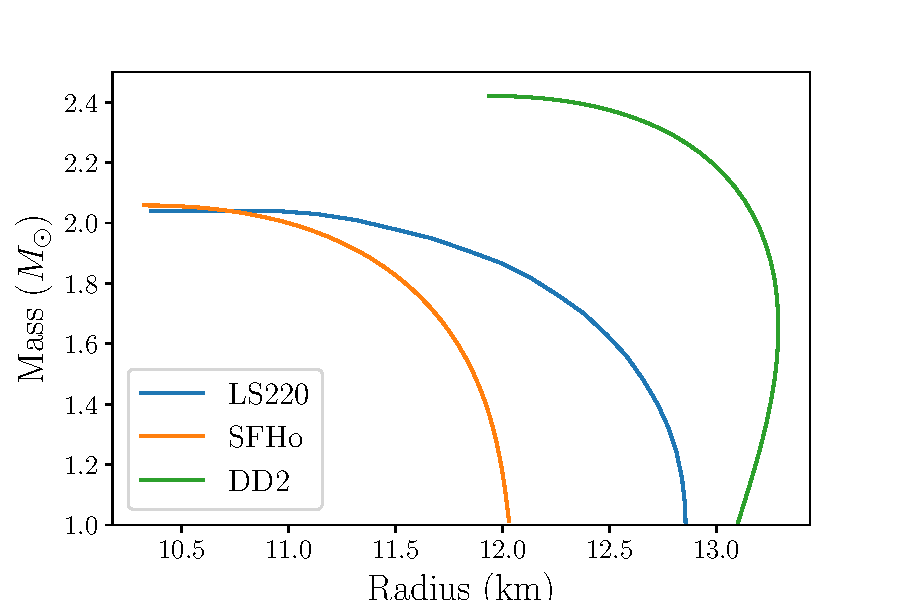
\includegraphics[width=.45\textwidth]{Figures/eos.png}
%% \fbox{\includegraphics[width=.495\textwidth,frame]{Figures/{-18ms_3d}.png}}\hfill
%%             \includegraphics[width=.495\textwidth,frame]{Figures/{-.3ms_3d}.png}\\
%%             \includegraphics[width=.495\textwidth,frame]{Figures/3ms_3d.png}\hfill
%%             \includegraphics[width=.495\textwidth,frame]{Figures/{7.5ms_3d}.png}
  
}
\subsection{GRRHD}
\frame{
  \frametitle{General Relativistic Radiation-Hydrodynamics}
}
\subsection{Ejecta Types}
\frame{
  \frametitle{Ejecta Types}
  \includegraphics[width=\textwidth]{./pictures/typesofejecta.png}
}
\subsection{Dynamical Ejecta}
\frame{
  \frametitle{Dynamical Ejecta}
}
\subsection{Secular Ejecta}
\frame{
  \frametitle{Secular Ejecta}
  %% \includegraphics[width=\textwidth]{Figures/{misc_tabular_3ms_2}.png}
  %% \includegraphics[width=.48\textwidth]{Figures/disk_masses.png}
}
\subsection{Velocity and Electron Fraction}
\frame{
  \frametitle{Velocity and Electron Fraction}

  %%   \includegraphics[width=.5\textwidth]{Figures/eos_12132_vinf_equa.eps}\\
  %% \includegraphics[width=.5\textwidth]{Figures/eos_12132_vinf_polar.eps}

  %% \includegraphics[width=.47\textwidth]{Figures/eos_12132_ye_equa.png}\\
  %% \includegraphics[width=.47\textwidth]{Figures/eos_12132_ye_polar.png}
  
  %% \includegraphics[width=.47\textwidth]{Figures/eos_sfho_vinf_equa.png}\\
  %% \includegraphics[width=.47\textwidth]{Figures/eos_sfho_vinf_polar.png}
  
  %% \includegraphics[width=.495\textwidth]{Figures/eos_sfho_ye_equa.png}\\
 %% \includegraphics[width=.495\textwidth]{Figures/eos_sfho_ye_polar.png}
}
\subsection{Neutrino Irradiation}
\frame{
  \frametitle{Neutrino Irradiation}
   %% \includegraphics[width=.45\textwidth]{Figures/s12132_7_5_and_10.png}
}
\subsection{Neutrino Emission}
\frame{
  \frametitle{Neutrino Emission}
  %% \centering \includegraphics[width=\textwidth,trim=300 0 300 0,clip=true]{Figures/eos_theta_hist_flux.pdf}
  %% \includegraphics[width=.45\textwidth]{Figures/eos-nulum-antionly.png}
  %% \includegraphics[width=.48\textwidth,trim=0 0 0 0,clip=true]{Figures/enua_slices.png}
  \includegraphics[width=\textwidth]{./pictures/chap3/Figures/dd2-nulum.png}
}
\subsection{Future work}
\frame{
  \frametitle{Future work}
}

%%%%%%%%%%%%%%%%%%%%%%%%%%%%%%%%%%%%%%%%%%%%%%%%%%%%%%%%%%%%
%
% Outline / Table of Contents
%
%%%%%%%%%%%%%%%%%%%%%%%%%%%%%%%%%%%%%%%%%%%%%%%%%%%%%%%%%%%%
% \section[Outline]{}
% \frame{\tableofcontents}

%%%%%%%%%%%%%%%%%%%%%%%%%%%%%%%%%%%%%%%%%%%%%%%%%%%%%%%%%%%%
%
% Sections
%
%%%%%%%%%%%%%%%%%%%%%%%%%%%%%%%%%%%%%%%%%%%%%%%%%%%%%%%%%%%%

%% \section{Background}

\subsection{Next-Gen G-Wave Astronomy}
\frame{
\frametitle{Next-Generation Gravitational Wave Astronomy}

\begin{columns}
  \begin{column}{.48\textwidth}
    Detector network by $\approx 2020$
    \begin{itemize}
\scriptsize 
    \item[\blacksquare]aLIGO (Washington State)
    \item[\blacksquare]aLIGO (Louisiana)
    \item[\blacksquare]aVIRGO (Italy)
    \item[\blacksquare]GEO-HF (Germany)
    \item[\blacksquare]KAGRA (Japan)
    \item[\blacksquare]LIGO-India
    \end{itemize}
\vspace{1cm}
Candidate Systems
\begin{itemize}
\scriptsize 
\item[\blacksquare]\scriptsize Binary Neutron Star (NS-NS)
\item[\blacksquare]\scriptsize Binary Black Holes (BH-BH)
\item[\blacksquare]\scriptsize Neutron Star - Black Hole (NS-BH)
\end{itemize}

  \end{column}
  \begin{column}{.48\textwidth}
\centering{\text{\tiny [Sathyaprakash
 2014]}}
   \includegraphics[width=.9\textwidth]{pictures/worldwide.pdf} \\
   \includegraphics[width=\textwidth]{pictures/abadie.pdf} \\
    \centering{\text{ \tiny [Abadie et al; 1003.2480]}}
  \end{column}
\end{columns}
}

\frame{
\frametitle{Binary Mergers}
\vspace{0cm}
\hspace{0cm}
\includegraphics[width=\textwidth]{pictures/shibata_cropped.pdf}\\
{\tiny Slide adapted from Shibata talk in 2011.}
}

\subsection{Constraining the NS EOS}
\frame{
\frametitle{Neutron Star Equation Of State (EOS)}

\begin{columns}
  \begin{column}{.48\textwidth}
\scriptsize {\boldmath$\text{EOS} \equiv P=P(\rho,T,Y_{e},..)$ still unknown.}\\
\vspace{.6cm}
   \includegraphics[width=\textwidth]{pictures/ns-crop.pdf} \\
\scriptsize {\vspace{.5cm}A realistic EOS captures microphysics in all theoretical regions.}\\

  \end{column}

  \begin{column}{.48\textwidth}

    \centering \tiny [Lattimer;1305.3510]
\vspace{.05cm}
\centering{ \includegraphics[width=.7\textwidth]{pictures/eos.pdf}} \\


\begin{mybox}{white}{\centering \scriptsize Spherical TOV Star}
\vspace{-.3cm}
\tiny    \begin{equation*}
      \label{eq:1}
      \begin{split}
        &\frac{dP}{dr} = -\frac{(G(m(r)) + 4\pi r^{3}P/c^{2})(\rho + P/c^{2})}{r(r-2Gm(r)/c^{2})} \\
& \frac{dm}{dr} = 4\pi\rho \\
&P = P(\rho, T, Y_{e}, ...)
      \end{split}
    \end{equation*}   
\end{mybox}
  \end{column}
\end{columns}
}

% \frame{
% \frametitle{Constraining the Equation Of State}

% \centering{
% \includegraphics[width=.4\textwidth]{pictures/shibata2.pdf} \\
% }

% % \begin{minipage}
% \begin{columns}

%   \begin{column}{.3\textwidth}
% \vspace{-4cm}
% \centering {   \includegraphics[width=\textwidth]{pictures/lambda.pdf}}
%   \end{column}
%   \begin{column}{.6\textwidth}
% \centering    \includegraphics[width=\textwidth]{pictures/f3.pdf} \\
%   \end{column}
% \end{columns}
% % \end{minipage}


% }


\begin{frame}
\frametitle{Constraining the Equation Of State Using GWs}
\begin{columns}
\column{0.5\textwidth}
\begin{minipage}[c][0.4\textheight][c]{\linewidth}
  \centering
\includegraphics[width=\textwidth]{pictures/shibata2.pdf}
\end{minipage}
\begin{minipage}[c][0.4\textheight][c]{\linewidth}
  \centering
 \includegraphics[width=.8\textwidth]{pictures/lambda.pdf}\\
{\tiny [Hinderer et al; 0911.3535]}
\end{minipage}
\column{0.5\textwidth}
\begin{minipage}[c][0.4\textheight][c]{\linewidth}
  \centering{\item[\blacksquare]\textbf{Two Interesting Phases.}}
  \begin{enumerate}
  \item[\blacksquare]Late Inspiral - Tidal Deformability $\lambda$
  \item[\blacksquare]Postmerger HNS - 3 peak frequencies
  \end{enumerate}
\end{minipage}
\begin{minipage}[c][0.4\textheight][c]{\linewidth}
  \centering
  \includegraphics[width=.7\textwidth]{pictures/f3.pdf}\\
\vspace{-.2cm}
{\tiny [Takami et al; 1412.3240]}
\end{minipage}
\end{columns}
\end{frame}

\subsection{SpECTRE: Next-Gen Numerical Relativity}

\frame{
\frametitle{Solving the Field Equations on a Computer}

Write Einstein's field equations as an initial-value problem for $g_{\mu\nu}$\\
\vspace{.5cm}
\begin{mybox}{white}{}
\begin{equation*}
\label{eq:3}
\vspace{.3cm}
\scriptsize
G_{\mu\nu} = 8\pi T_{\mu\nu} \rightarrow \begin{cases}
    \text{Constraints} &  (\text{like  } \nabla \cdot B = 0)\\
    \text{Evolution Equations} & (\text{like  } \partial_{t} B = -\nabla \times E)
\end{cases}
\end{equation*}
\end{mybox} 
\vspace{.3cm}
Obtain a computer cluster and \\
\vspace{.3cm}
\begin{mybox}{white}{}
\begin{enumerate}
\item[1.]Solve constraints ({\bf initial-data equations}) at t = 0
  \begin{itemize}
  \item[--] 4  coupled nonlinear 2nd-order elliptic PDEs
  \end{itemize}
\item[2.]Time-step forward with evolution equations
  \begin{itemize}
  \item[--] 50 coupled nonlinear 1st-order hyperbolic PDEs
  \end{itemize}
% \item[\blacksquare]Use constraints to check quality of the evolution
\end{enumerate}
\end{mybox}
% \begin{itemize}
% \item[\blacksquare]Solve constraints (initial-data equations) at t = 0
% \begin{itemize}
% \item[--] 4 (or 5) coupled non-linear 2nd-order elliptic PDEs
% \end{itemize}}
% \item[\blacksquare]Advance initial data in time using evolution equations
% \begin{itemize}
% \item[--] 50 coupled non-linear 1st-order hyperbolic PDEs
% \end{itemize}
% \end{itemize}
}

\frame{
\frametitle{SpEC @ black-holes.org}

\begin{columns}
  \begin{column}{.48\textwidth}
\scriptsize
    \begin{itemize}
    \item[\blacksquare]The Spectral Einstein Code (SpEC) is a multi-domain spectral code for solving the Einstein field equations written primarily by \textbf{Larry Kidder, Harald Pfeiffer} and \textbf{Mark Sheel}.
    \item[\blacksquare]The SpEC code was initially written for BBH systems.
    % \item[\blacksquare]Realistic NSNS and NSBH simulations are hard in SpEC due to:
    \end{itemize}
\vspace{.5cm}
\begin{mybox}{white}{\centering NSNS/NSBH are hard due to}
      \begin{itemize}[leftmargin=*]
\scriptsize
    \item[1.] SpEC scales to only 50-300 cores. Need lots of cores for accurate microphysics.
    \item[2.] Spectral methods cannot \\ handle discontinuities/shocks \\easily.
      \end{itemize}
\end{mybox}
  \end{column}
  \begin{column}{.48\textwidth}
\begin{center}
% \vspace{-.2cm}
\includegraphics[width=\textwidth]{pictures/sxsfamily.pdf} \\ \vspace{.5cm}
    \includegraphics[width=\textwidth]{pictures/catalog.pdf} \\ 
{\tiny [174 simulations; Mroue et al; 1304.6077]}
\end{center}
  \end{column}

\end{columns}


}


\frame{
\frametitle{SpECTRE: Next-Generation Numerical Relativity}

\begin{center}
\includegraphics[width=.5\textwidth]{pictures/spectre.png} \\ 

\end{center}
\vspace{-.8cm}
\begin{columns}
  \begin{column}{.48\textwidth}
\begin{center}
    \begin{block}{\centering Science Goals}
\begin{itemize}
\scriptsize
      \item[\blacksquare]full GR
      \item[\blacksquare]neutrino-radiation-MHD
      \item[\blacksquare]temperature dependent EOS
\end{itemize}
    \end{block}
\end{center}
  \end{column}
  \begin{column}{.48\textwidth}
\begin{center}
    \begin{block}{\centering Computational Goals}
      \begin{itemize}
\scriptsize
\item[\blacksquare]Scale to O(100k) Cores
\item[\blacksquare]Discontinuous Galerkin
\item[\blacksquare]Open-Source      
      \end{itemize}
    \end{block}
\end{center}
  \end{column}

\end{columns}
\begin{tcolorbox}
\textbf{Primary Goal of PhD Thesis:} Write the SpECTRE Elliptic Solver for realistic NSNS/NSBH initial data. 
\end{tcolorbox}
{\tiny Logo From Upcoming James Bond Film}  
}

\subsection{Problems With Current Initial-Data Solvers}
\frame{
\frametitle{Problems With Current Initial-Data Solvers}

\begin{columns}
  \begin{column}{.48\textwidth}

\scriptsize The majority of NSNS simulations in the literature use polytropes or
at best, \textbf{piecewise polytropes} for stars with \textbf{low compactness} $C=M_{NS}/R_{NS} \approx .1$
\vspace{.5cm}
\begin{mybox}{white}{\centering Piecewise Polytrope}
\vspace{-.5cm}
\centering
\begin{equation*}
  P = K_{i}\rho^{\Gamma_{i}}; \,\,\,\, \rho_{i} < \rho < \rho_{i+1}
\end{equation*}
\includegraphics[width=\textwidth]{pictures/iloveq-crop.pdf}\\
\vspace{.2cm}
\centering
{\tiny [Yagi et al; 1406.7587]}
\end{mybox}
  \end{column}
  \begin{column}{.48\textwidth}
    \includegraphics[width=\textwidth]{pictures/fabertable_cropped.pdf}\\
\vspace{-.2cm}
\centering{{\tiny [Faber et al; lrr-2012]}}\\
\vspace{.5cm}
\begin{tcolorbox}
\scriptsize For realistic waveform models, we need initial-data with 
\begin{itemize}
\item[\blacksquare]temperature-dependent, realistic EOS
\item[\blacksquare]any compactness
\end{itemize}

Current Solvers (SpEC, LORENE) have difficulties in this regime.
\end{tcolorbox}    
  \end{column}
\end{columns}



}



%%% Local Variables:
%%% mode: latex
%%% TeX-master: "../main"
%%% End:

%% \section{SpECTRE Elliptic Solver}

\subsection{Overview}
\frame{
\frametitle{SpECTRE Elliptic Solver}
\begin{center}
      \includegraphics[width=.8\textwidth]{pictures/spectrells.pdf}\\
  \begin{block}{\centering Components}
\begin{itemize}
\scriptsize
\item[\blacksquare]PDE Discretization: \textbf{Discontinuous Galerkin}
\item[\blacksquare]Adaptive Mesh Refinement: \textbf{hp-AMR}
\item[\blacksquare]Parallel Mesh Storage  \textbf{Parallel Forest of Octrees}
\item[\blacksquare]Linear system solver: \textbf{Multigrid Preconditioner + PETSc Iterative solver}
\item[\blacksquare]Visualization: \textbf{yt}
\end{itemize}   
  \end{block}
\end{center}
}

\subsection{Discontinuous Galerkin}
\frame{
  \frametitle{Traditional Discretization Schemes}

{\scriptsize
Finite difference and Spectral Finite Elements are currently used.
We write the PDE as

\begin{equation*}
\label{eq:1}
\begin{split}
&R(u) = 0 \\
\rightarrow &R_{h}(u) \approx 0 \text{    (on a computer)}
\end{split}
\end{equation*}
}
  \begin{columns}
    \begin{column}{.48\textwidth}
% First formulated in 1970, dG methods were largely ignored until recently.
% \vspace{1cm} 
%       \begin{block}{Advantages of dG}
%         \begin{enumerate}
%         \item[\blacksquare]hp-adaptive
%         \item[\blacksquare]easily parallelized
%         \item[\blacksquare]conceptually similar in n-d
%         \item[\blacksquare]small local operators
%         \item[\blacksquare]different numerical fluxes
%         \end{enumerate}
      % \end{block}
\begin{mybox}{white}{\centering Finite Difference}
% \centering \scriptsize \underline {Finite Difference}\\
\scriptsize
\begin{itemize}
\item[\blacksquare]Simple to code 
\item[\blacksquare]Algebraically convergent
\end{itemize}
      \begin{center} \includegraphics[width=.85\textwidth]{pictures/fd.pdf}\\
\end{center}
\end{tcolorbox}
    \end{column}
    \begin{column}{.48\textwidth}
\begin{mybox}{white}{\centering Spectral FEM}
% \centering \scriptsize  \underline {Spectral FEM}\\
\scriptsize
\begin{itemize}
\item[\blacksquare]Hard to code 
\item[\blacksquare]Exponentially convergent
\end{itemize}
      \includegraphics[width=\textwidth]{pictures/spectral.pdf}      
\end{mybox}
    \end{column}
  \end{columns}

}

\frame{
  \frametitle{Discontinuous Galerkin (DG)}

  \begin{columns}
    \begin{column}{.48\textwidth}
$\,\,$\\
\vspace{.5cm}
First used in 1970 by \\ Reed and Hill. \\ 
\vspace{.2cm}
DG methods were largely ignored until recently.\\
\vspace{.3cm} 
\begin{mybox}{white}{\centering Discontinuous Galerkin}
      \includegraphics[width=\textwidth]{pictures/dg2.pdf}      \\
\end{mybox}
    \end{column}
    \begin{column}{.48\textwidth}
      \includegraphics[width=\textwidth]{pictures/dg.pdf}\\
\vspace{-.2cm}
\centering {\tiny  [Di Pietro, Ern; Springer 2012]}
      \begin{block}{\centering Advantages of dG}
        \begin{enumerate}
        \item[\blacksquare]hp-adaptive
        \item[\blacksquare]easily parallelized
        \item[\blacksquare]conceptually similar in n-d
        \item[\blacksquare]small local operators
        \end{enumerate}
      \end{block}
    \end{column}
  \end{columns}

}

\subsection{hp-AMR}
\begin{frame}
\frametitle{Adaptive Mesh Refinement}
\begin{columns}
  \begin{column}{.6\textwidth}
% \begin{itemize}
% \item[\blacksquare]BNS length scales:
\begin{center}
\vspace{.5cm}
\setul{}{2pt}
\ul{NSNS Coalescence Length Scales}
\vspace{.3cm}
  \begin{enumerate}
  \item[\blacksquare] internal NS dynamics\footnote[frame]{\scriptsize Assuming Polytropic EOS} $\approx 0.1M_{NS}$ 
  \item[\blacksquare] evolution time scale $\approx 0.1M_{NS}$
  \item[\blacksquare] orbital separation $\approx 50M_{NS}$
  \item[\blacksquare] wave zone boundary $\approx 1000M_{NS}$
  \end{enumerate} 
\end{center}
\vspace{1cm}
  \end{column}
  \begin{column}{.35\textwidth} 
\begin{center}
\includegraphics[width=\textwidth]{pictures/ns_amr.pdf}
\vspace{-.15cm}   
\text{ \scriptsize [Evans et al; gr-qc/0501066]}
\end{center}
% \vspace{.5cm}
    % \includegraphics[width=\textwidth, height=.7\textwidth]{pictures/nbody_wakes_cropped.pdf}
  \end{column}
\end{columns}

\end{frame}

\frame{
\frametitle{hp-Adaptive Mesh Refinement}

\begin{mybox}{white}{}
\centering {dG naturally allows for hp-adaptivity}\\
\end{mybox}
\vspace{.1cm}

\begin{columns}
  \begin{column}{.48\textwidth}
\centering
% \begin{itemize}
% \item[\blacksquare]BNS length scales:
\begin{itemize}
\item[\blacksquare] \textbf{h-refinement} for discontinuous regions \\
\vspace{.75cm}
\includegraphics[width=.8\textwidth]{pictures/hrefine.pdf} \\
 \end{itemize}
\vspace{.5cm}
\centering \includegraphics[width=.7\textwidth]{pictures/hermes1.pdf} \\


% \end{itemize}    
  \end{column}
  \begin{column}{.48\textwidth} 
\begin{center}
% \tiny{advection-reaction problem with hp-AMR}
 % \includegraphics[width=\textwidth]{pictures/hermes1.pdf} \\   
\vspace{-.4cm}
\begin{itemize}
 \item[\blacksquare]\textbf{p-enrichment} for smooth regions \\
\vspace{.65cm}
\includegraphics[width=.8\textwidth]{pictures/prefine.pdf} \\
\end{itemize}
\vspace{.3cm}
 \includegraphics[width=.6\textwidth]{pictures/hermes2.pdf} \\
\end{center}
% \vspace{.5cm}
    % \includegraphics[width=\textwidth, height=.7\textwidth]{pictures/nbody_wakes_cropped.pdf}
  \end{column}
\end{columns}
\vspace{.2cm}   
\centering \text{ \scriptsize [hpfem.com/hermes]}
  % discontinuous Galerkin naturally allows for hp-AMR
}

\subsection{Forest of Octrees}
\frame{
\frametitle{p4est: Parallel AMR on a Forest of Octrees}
    \begin{itemize}
    \item[\blacksquare]distributed octrees for PDE meshes
    \item[\blacksquare]load balancing
    \item[\blacksquare]scale-tested on $O(500k)$ cores
    \end{itemize}
\begin{columns}
  \begin{column}{.48\textwidth}

    \begin{center}
\includegraphics[width=\textwidth]{pictures/earthmantle_cropped.pdf}\\
\vspace{-.4cm}  
{\tiny Mantle simulation with 24-octrees.}      
    \end{center}

  \end{column}
\begin{column}{.4\textwidth} 
    \begin{center}
\includegraphics[width=\textwidth]{pictures/p4esttrees_cropped.pdf}\\
% \includegraphics[width=\textwidth]{pictures/p4estblocks_cropped.pdf}\\
\includegraphics[width=\textwidth]{pictures/p4estblocks_cropped.pdf}
\vspace{-.3cm}  
{ \tiny [Burstedde et al; 1406.0089]}
   \end{center}
\end{column}
\end{columns}

}

% \begin{frame}
% \frametitle{p4est: Scaling Example}
% \label{sec-2-2}
% \begin{columns}
% \begin{column}{.4\textwidth}
% %% Column 1
% \label{sec-2-2-1}

% \tiny Sundar, Hari, et al. ``Parallel geometric-algebraic multigrid on unstructured forests of octrees.'' Proceedings of the International Conference on High Performance Computing, Networking, Storage and Analysis. IEEE Computer Society Press, 2012.
% \begin{block}{\small Variable Coefficient Poisson}
% \label{sec-2-2-2}

%      \vspace{-.5cm}
%      \begin{equation*}
%      \begin{split}
%      & \nabla \cdot (\mu( \vec x) \nabla u ( \vec x) ) = f(x)  \,\,\,\, \vec x \in \Omega \\
%      & u(\vec x ) = 0 \,\,\,\, \vec x \in \partial \Omega \\
%      \end{split}
%      \end{equation*}
% \centering \includegraphics[width=.6\textwidth]{pictures/finegrid_gmg.png}
% \end{block}
% \end{column}
% \begin{column}{.48\textwidth}
% %% Column 1
% \label{sec-2-2-3}
% \begin{block}{\small \centering Weak Scaling}
% \label{sec-2-2-4}

% \centering \includegraphics[width=\textwidth]{pictures/weak_scaling_sphere.png}
% \end{block}
% \begin{block}{\small \centering Strong Scaling}
% \label{sec-2-2-5}

% \centering \includegraphics[width=\textwidth]{pictures/strong_scaling_sphere.png} \\
% \end{block}
% \end{column}
% \end{columns}
% \end{frame}


\subsection{Multigrid + Iterative Solver}
\label{subsec:label}
\frame{
  \frametitle{Multigrid + Krylov Iteration}

\textbf{Once discretized, elliptic PDEs boil down to:}
\begin{center}
\begin{minipage}{5cm}
\begin{block}{\centering $N \times N$ Linear System}
\centering{$Au=b$}
\end{block}
\end{minipage}
\end{center}
\scriptsize
\vspace{.5cm}
\centering{\textbf {Two Main Solution Methods}}
\begin{columns}
  \begin{column}{.55\textwidth}
    \begin{block}{\centering Direct Methods}
      % \begin{}
\centering{$u = A^{-1}b$}
      % \end{equation*}
      \begin{itemize}
      \item[\blacksquare]$O(N^{2})$ storage
      \item[\blacksquare]no pre-conditioning 
      \item[\blacksquare]ruins operator locality
      \end{itemize}

    \end{block}
  \end{column}
  \begin{column}{.4\textwidth}
% \vspace{-.92cm}
    \begin{block}{\centering Iterative Methods}
      % \begin{equation*}
        \centering{$u_k = u_{k-1} + \alpha d_{k}$}
      % \end{equation*}
\begin{itemize}
      \item[\blacksquare]$O(N)$ storage
      \item[\blacksquare]pre-conditioning
      \item[\blacksquare]preserves operator locality
\end{itemize}
    \end{block}
  \end{column}
\end{columns}

\begin{mybox}{white}{}
\centering \bf Optimal combination: Multigrid preconditioner + Iterative Solver \\
{\tiny [Wathen; 2015]}
\end{mybox}
}

% \frame{
%   \frametitle{Multigrid Preconditioner}

% {\scriptsize Preconditioning is a technique for minimizing $\kappa(A) = \frac{\lambda_{max}}{\lambda_{min}}$.}

% % \textbf{Once discretized, elliptic PDEs boil down to:}
% \vspace{-.5cm}
% \begin{center}
% \begin{minipage}{5cm}
% \begin{block}{\centering Preconditioning}
% \centering{$M^{-1}Ax=M^{-1}b$}
% $\kappa(M^{-1}A) \ll \kappa(A)$
% \end{block}
% \end{minipage}
% \end{center}

% {\scriptsize The most robust, scalable pre-conditioner known is multigrid [Wathen et al; 2015].}

% % \includegraphics[width=\textwidth]{pictures/multigrid.pdf}\\
% % \begin{block}{\centering [Tatebe et al; 1994]}
% \vspace{.5cm}
%   \begin{columns}

%     \begin{column}{.4\textwidth}
% \centering{

% \begin{block}{\centering [Tatebe et al; 1994]}
% \vspace{-.3cm}
%   \begin{equation*}
%     \nabla (k \nabla u) = f \\ \\
%   \end{equation*}

%   \vspace{-2cm}
% \begin{equation*}
% \label{eq:4}
% \tiny
% \begin{split}
%  \Omega &\equiv [0,1] \times [0,1] \\
% u &\equiv 0 \,\,\, on \,\,\, \partial \Omega \\
% k &\equiv \text{discontinuous function} \\
% f &\equiv \text{discontinuous function} \\
% \end{split}
% \end{equation*}
% \end{block}
% % \normalsize
% }
%       % $- $ 
%       % $ \Omega \equiv [0,1] \times [0,1]$ \\ \\
% % $u \equiv 0$ on $\partial \Omega$\\
% % }
% % k,f are discontinuous
%     \end{column}
%     \begin{column}{.55\textwidth}
%       \centering \fbox{\includegraphics[width=\textwidth]{pictures/MGCG_cropped.pdf}}
%     \end{column}
%   \end{columns}
% % \end{block}
% }


\subsection{yt visualization}
\label{subsec:label}
\frame{
  \frametitle{yt visualization @ yt-project.org}
\begin{columns}
  \begin{column}{.48\textwidth}
$\,\,\,$\\
\vspace{.2cm}
\includegraphics[scale=0.04]{pictures/ytlogo.png}
{\small \, is a python package for}
\centering
{\small visualizing volumetric, }
{\small multi-resolution data from}
{\small astrophysical simulations. } \\
\vspace{.8cm}
\includegraphics[width=\textwidth]{pictures/ji1_cropped.pdf}\\

  \end{column}
\begin{column}{.48\textwidth} 

% \includegraphics[width=\textwidth]{pictures/p4estblocks_cropped.pdf}\\
\includegraphics[width=\textwidth,height=.5\textwidth]{pictures/ytlines.png} \\
\vspace{.6cm}
\includegraphics[width=\textwidth]{pictures/ji2_cropped.pdf}
\end{column}
\end{columns}
\begin{center}{ \tiny [White dwarf merger. Left: Magnetic field lines. Right: $\beta=$ Gas Pressure/Magnetic Pressure. Ji et al; 2013]}\end{center}
}

%%% Local Variables:
%%% mode: latex
%%% TeX-master: "main"
%%% End:

%% \section{Plan and Timeline}
\label{sec:label}
\subsection{Plan and Timeline: Overview}

\frame{
\frametitle{Plan and Timeline: Overview}

\scriptsize
The plan is to take my current code and make incremental changes to get to the end goal of realistic NSNS/NSBH initial-data. At each stage, attack an interesting initial-data problem and write a paper.

\vspace{.3cm}

\begin{mybox}{white}{\centering \url{https://github.com/trevor-vincent/p4est_dG_multigrid/}}
 % \\
% \begin{center}
% \begin{mybox}{white}{}
% \begin{center}
   
% \end{center}
% \vspace{-1cm}
% \begin{center}
\begin{columns}
  \begin{column}{.48\textwidth}
\vspace{-.2cm}
\begin{mybox}{white}{\tiny \centering Components so far}
\begin{itemize}[leftmargin=*]
\tiny
\item[\blacksquare]discontinuous Galerkin
\item[\blacksquare]p4est with 2-D mesh
\item[\blacksquare]conjugate gradient Krylov solver
\end{itemize}
\end{mybox}
% \begin{mybox}{white}{}
\vspace{.03cm}
\includegraphics[width=\textwidth]{pictures/Kfixed.pdf}
% \end{mybox}     \\
% \vspace{.5cm}

  \end{column}
  \begin{column}{.48\textwidth}
{\tiny $\,\,\,$}\\
{\tiny $\,\,\,$}\\
{\tiny Below: Exponential and Algebraic convergence for a simple Poisson problem with h and p fixed respectively.}
% \vspace{.4cm}
% \begin{mybox}{white}{}
\vspace{-.3cm}
\includegraphics[width=\textwidth]{pictures/Nfixed.pdf}        
% \end{mybox}
  \end{column} 
\end{columns}


% \end{center}       
\end{mybox}

% and make incremental changes.





}

\subsection{Phase 1}

\frame{
  \frametitle{Phase 1.1: Puncture Initial Data}



\begin{columns}
  \begin{column}{.58\textwidth}
\scriptsize
\begin{mybox}{white}{\centering Multi-Black Hole Initial Data}
\begin{itemize}[leftmargin=*]
\item[\blacksquare]Each black hole is represented as a puncture in the manifold. 
\item[\blacksquare]3 of the 4 vacuum constraint equations are analytically solvable. 
\item[\blacksquare]Spins and momenta, $S^i$ and $P^{i}$ come in as free variables.
% \item[\blacksquare]Last remaining constraint equation:
\end{itemize}
\begin{equation*}
\label{eq:8}
-(\partial^2_x+\partial^2_y+\partial^2_z)u = \frac{1}{8}\Hat K^{ij} \Hat K_{ij} + 2\pi\rho\psi^{-3}. 
\end{equation*}
\end{mybox}
    \begin{mybox}{white}{\centering Estimated Time}
\centering {Mid-June to October 1st 2015}
\end{mybox}
  \end{column}
  \begin{column}{.4\textwidth}
    \begin{mybox}{white}{\centering \tiny Important Aspects of Stage}
\begin{itemize}[leftmargin=*]
\tiny
\item[\blacksquare]Can test scaling by placing third BH far away for BBH
\item[\blacksquare]nice test of hp-adaptivity \\($C^{4}$ smooth around punctures)
 \item[\blacksquare]scaling results/code debut in publication
\end{itemize}
% \hspace{-.5cm}
\end{mybox}
    \begin{mybox}{white}{\centering  \tiny Code Changes}
\tiny
\begin{itemize}[leftmargin=*]
\item[\blacksquare]add multigrid to 2-D code
\item[\blacksquare]convert to 3-D
\item[\blacksquare]add non-linear solver from PetSC
\item[\blacksquare]hp-adaptive mesh refinement
% \item[\blacksquare]three black-hole puncture initial data
% \item[\blacksquare]weak/strong scaling tests
% \item[\blacksquare]publication
\end{itemize}
\end{mybox}
  \end{column}
\end{columns}

}

\frame{
  \frametitle{Phase 1.2: TOV Initial Data in 3D}


\begin{columns}
  \begin{column}{.63\textwidth}
\scriptsize
\begin{mybox}{white}{\centering TOV Initial Data in 3D with EOS tables}
\begin{itemize}[leftmargin=*]
% \item[\blacksquare]Solve the TOV Initial-Data equations in 3-D. 
% \item[\blacksquare]Using a tabulated EOS 
\end{itemize}
\begin{equation*}
\label{eq:9}
\begin{split}
  &\frac{dp}{dr} = -G(\rho(1+\epsilon/c^{2}) + p/c^2) \frac{m + 4\pi r^{3} p/c^2}{r(r-2Gm/c^{2})}, \\
  &\frac{dm}{dr} = 4\pi r^2 \rho (1 + \epsilon/c^2), \\
  &\frac{d \ln(\alpha)}{dr} = \frac{m+4\pi r^{3}p/c^2}{r(r-2Gm/c^{2})}, \\
  &P = P(\rho) \,\,\,\,\,\, \text{(from table)}.
\end{split}
\end{equation*}
\end{mybox}
    \begin{mybox}{white}{\centering Estimated Time}
\centering October 1st to December 31st, 2015
\end{mybox}
  \end{column}
  \begin{column}{.4\textwidth}
    \begin{mybox}{white}{\centering \tiny Important Aspects of Stage}
\begin{itemize}[leftmargin=*]
\tiny
\item[\blacksquare]Tests hp-AMR against discontinuities with unknown location
\item[\blacksquare]Tests p4est on non-cubic domain
\item[\blacksquare]Required step for superimposed TOV initial-data
\end{itemize}
% \hspace{-.5cm}
\end{mybox}
    \begin{mybox}{white}{\centering  \tiny Code Changes}
\tiny
\begin{itemize}[leftmargin=*]
\item[\blacksquare] non-cubic domains
\item[\blacksquare] add yt visualization
% \item[\blacksquare]three black-hole puncture initial data
% \item[\blacksquare]weak/strong scaling tests
% \item[\blacksquare]publication
\end{itemize}
\end{mybox}
  \end{column}
\end{columns}
}


\subsection{Phase 2}

\frame{
  \frametitle{Phase 2: NS-\{NS,BH\} Initial-Data with Moderate C}

\begin{columns}
  \begin{column}{.58\textwidth}
\scriptsize
\centering
\begin{mybox}{white}{\centering \text{NS-\{NS,BH\}} + Moderate Compactness}
\begin{itemize}[leftmargin=*]
\item[\blacksquare]Solve the full Constraint Equations in 3D. 
\item[\blacksquare]Using a tabulated EOS with moderate compactness.
\end{itemize}
\end{mybox}
    \begin{mybox}{white}{\centering Estimated Time}
\centering January 1st to March 1st, 2016.
\end{mybox}
  \end{column}
  \begin{column}{.4\textwidth}
    \begin{mybox}{white}{\centering \scriptsize \tiny Important Aspects of Stage}
\begin{itemize}[leftmargin=*]
\scriptsize
\item[\blacksquare]can compare to SpEC results {\tiny [Henriksson et al; 2014]}
\item[\blacksquare]Publication detailing results
\end{itemize}
% \hspace{-.5cm}
\end{mybox}
%     \begin{mybox}{white}{\centering  \tiny Code Changes}
% \tiny
% \begin{itemize}
% \item[\blacksquare]add yt visualization
% % \item[\blacksquare]three black-hole puncture initial data
% % \item[\blacksquare]weak/strong scaling tests
% % \item[\blacksquare]publication
% \end{itemize}
% \end{mybox}
  \end{column}
\end{columns}

}


\subsection{Phase 3}

\frame{
  \frametitle{Phase 3: NS-\{NS,BH\} Initial-Data with High C}

\begin{columns}
  \begin{column}{.58\textwidth}
\scriptsize
\begin{mybox}{white}{\centering \text{NS-\{NS,BH\}} + High Compactness}
\begin{itemize}[leftmargin=*]
\item[\blacksquare]Solve the full Constraint Equations in 3D. 
\item[\blacksquare]Using tabulated EOSs and high compactness.
\item[\blacksquare]Extra schemes/constraints will have to be investigated in order to
get convergence
\end{itemize}
\end{mybox}
    \begin{mybox}{white}{\centering Estimated Time}
\centering June 1st, 2016 onwards.
\end{mybox}
  \end{column}
  \begin{column}{.4\textwidth}
    \begin{mybox}{white}{\centering \tiny Important Aspects of Stage}
\begin{itemize}[leftmargin=*]
\tiny
\item[\blacksquare]First ever initial-data in this regime
\item[\blacksquare]Publication detailing results
\end{itemize}
% \hspace{-.5cm}
\end{mybox}
%     \begin{mybox}{white}{\centering  \tiny Code Changes}
% \tiny
% \begin{itemize}
% \item[\blacksquare]add yt visualization
% % \item[\blacksquare]three black-hole puncture initial data
% % \item[\blacksquare]weak/strong scaling tests
% % \item[\blacksquare]publication
% \end{itemize}
% \end{mybox}
  \end{column}
\end{columns}

}


\subsection{Phase 4}

\frame{
  \frametitle{Phase 4: Other Simulations}

\begin{columns}
  \begin{column}{.58\textwidth}
\scriptsize
\begin{mybox}{white}{Newtonian Gravity Simulations}
\begin{itemize}[leftmargin=*]
\item[\blacksquare]With a powerful Elliptic Solver, other physics can be investigated. 
\item[\blacksquare]Newtonian gravity simulations (binary mergers with complex microphysics, galactic dynamics)
\end{itemize}
\end{mybox}
    \begin{mybox}{white}{\centering Estimated Time}
\centering Left-over/Unknown
\end{mybox}
  \end{column}
 %  \begin{column}{.4\textwidth}
%     \begin{mybox}{white}{\centering \tiny Important Aspects of Stage}
% \begin{itemize}
% \tiny
% \item[\blacksquare]First ever initial-data in this regime
% \item[\blacksquare]Publication detailing results
% \end{itemize}
% % \hspace{-.5cm}
% \end{mybox}
% %     \begin{mybox}{white}{\centering  \tiny Code Changes}
% % \tiny
% % \begin{itemize}
% % \item[\blacksquare]add yt visualization
% % % \item[\blacksquare]three black-hole puncture initial data
% % % \item[\blacksquare]weak/strong scaling tests
% % % \item[\blacksquare]publication
% % \end{itemize}
% % \end{mybox}
%   \end{column}
\end{columns}

}

\frame{

\frametitle{Questions?}

\begin{columns}
\begin{column}{.48\textwidth}
\begin{center}
\includegraphics[width=.6\textwidth]{pictures/2bh.pdf}\\
\vspace{.1cm}
{\centering \tiny [BBH; Lovelace et al]}\\
\vspace{.2cm}
\includegraphics[width=.6\textwidth]{pictures/rezzolla.pdf}\\
\vspace{.2cm}
{\centering \tiny [NSNS; Rezzolla et al]}
\end{center}
\end{column}
\begin{column}{.48\textwidth}
\begin{center}
\includegraphics[width=.5\textwidth]{pictures/francois.pdf}\\
\vspace{.1cm}
{\centering \tiny [NSBH; Foucart et al]}\\
\vspace{.2cm}
\includegraphics[width=.5\textwidth]{pictures/ott.png}\\
% \vspace{.2cm}
{\centering \tiny [Supernova; Ott et al]}
\end{center}
\end{column}
\end{columns}

}

%%% Local Variables:
%%% mode: latex
%%% TeX-master: "main"
%%% End:


%%%%%%%%%%%%%%%%%%%%%%%%%%%%%%%%%%%%%%%%%%%%%%%%%%%%%%%%%%%%
%
% References
%
%%%%%%%%%%%%%%%%%%%%%%%%%%%%%%%%%%%%%%%%%%%%%%%%%%%%%%%%%%%%

% \frame{\frametitle{References}
% \scriptsize
% \bibliographystyle{ieeetr}
% \bibliography{refs}
% \nocite{*}
% }

\end{document} 
